\graphicspath{{images/act_2.2/}}
\subsection{Gravity and Coriolis compensation}
The objective of this activity is analyze effects of gravity and Coriolis terms on the dynamics relation between interaction forces ($\fext$) and Cartesian configuration ($\cartesianconfiguration$). For this purpose, a simulation environment is developed that contains the UR5 robot and allows external forces to be applied. The simulation starts with robot end-effector cartesian position $\mathbf{p_0}=\begin{bmatrix}  0.577 &   0.192 &   0.364 \end{bmatrix}$~m. Then, external force $\mathbf{f_{ext}}= 50\sin{(2\pi t)}$ N is applied to robot end-effector. Finally, motion control is made up of two approaches: cartesian proportional-derivative impedance with gravity and Coriolis compensation (PDI+b) control and projection of the null space. In this sense, cartesian PDI+b control method focuses on set desired dynamic behavior and the projection of null space maintains the articular position close to $\mathbf{q_0}$. Finally, control law can be computed as 
\begin{equation}
	\boldsymbol{\tau}
	= \mathbf{J^T} (\mathbf{K_{des} e} + \mathbf{D_{des} \dot{e}} + \boldsymbol{\mu}) + \mathbf{N} \left(\mathbf{K_q(q_0-q) - D_q \dot{q}} \right),
	\label{eq:cartesian_PDI_b_N}
\end{equation}
\begin{align*}
	\boldsymbol{\Lambda} &= (\mathbf{J M^{-1} J^{T}})^{-1}, \\
	\boldsymbol{\mu} &= \mathbf{J^{T\#}} - \boldsymbol{\Lambda}\mathbf{\dot{J}\dot{q}}, \\
	\mathbf{N} &=(\mathbf{I_{6 \times 6}} - \mathbf{J^{\#} J} ),
\end{align*}

\noindent where $\mathbf{J}$ is geometric jacobian matrix, $\mathbf{e}=\mathbf{p_{des} - p}$ is end-effector position error, and $\mathbf{K_{des}, D_{des}}$ are desired stiffness and damping, respectively; $\mathbf{J^{\#}}$ is jacobian damped pseudo-inverse, $\boldsymbol{\mu}$ is nonlinear effects vector at Cartesian space, $\mathbf{N}$ is the null space projection of $\mathbf{J^{\#}}$, and $\mathbf{K_q, D_q}$ are the proportional and derivative gains for null space projection. 

Figure \ref{fig:act2.2_external_force_vs_cartesian_configuration} shows the dynamics relation between external torque ($\tauext$) and cartesian configuration ($\jointconfiguration$) using control law \eqref{eq:cartesian_PDI_b_N} with $\mathbf{K_{des}}=500\eye$ and $\mathbf{D_{des}}=50\eye$. In these figures, similar dynamic behaviors are observed in Cartesian position graphs due to compensation for gravitational and Coriolis effects. However, in the velocity and acceleration graphs, differences are observed at the beginning and at the end. Finally, impedance profiles can be improved by compensating for inertia at control law.

\begin{figure}
\centering
\subfloat[]{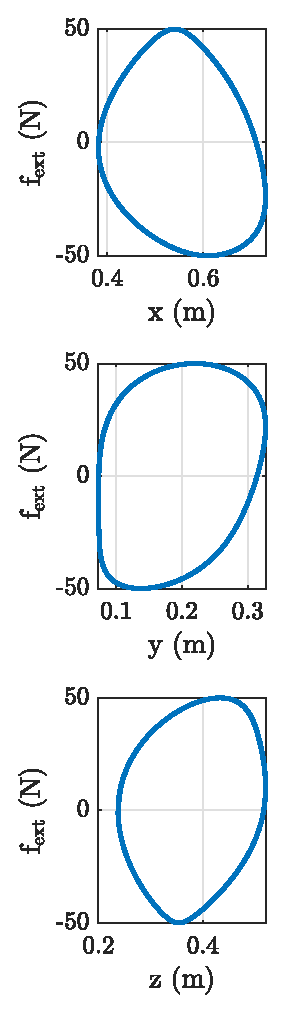
\includegraphics{external_force_vs_cartesian_position.eps} \label{fig:act2.2_force_vs_p}}
\subfloat[]{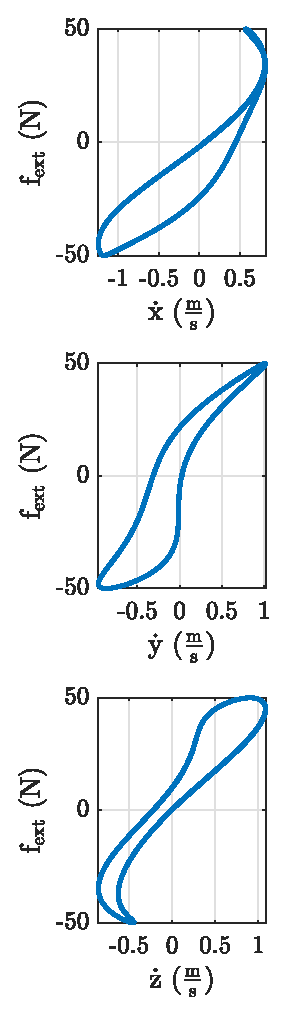
\includegraphics{external_force_vs_cartesian_velocity.eps} \label{fig:act2.2_force_vs_dp}}
\subfloat[]{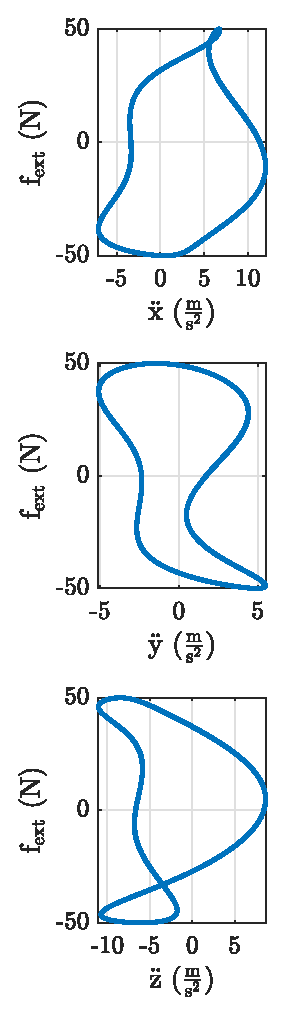
\includegraphics{external_force_vs_cartesian_acceleration.eps} \label{fig:act2.2_force_vs_ddp}}
\caption{Dynamics relation between external force ($\fext$) and Cartesian configuration ($\cartesianconfiguration$) using proportional-derivative impedance control \eqref{eq:cartesian_PDI_N} with $\mathbf{K_{des}}=500\eye$ and $\mathbf{D_{des}}=50\eye$: (a) position, (b) velocity and (c) acceleration.}
\label{fig:act2.2_external_force_vs_cartesian_configuration}
\end{figure}


